\section{Asymptotic freedom and the gluon*}
\label{sec:asymptotic_freedom}
We briefly discussed in Appendix~\ref{sec:force_range} that the particular strength of a force
is not a quantity that remains constant with energy. For example, the weak interaction is only weak at large distances (low energies) however at short range (high energy) it is stronger than the EM interaction. Consider the diagram below

\begin{center}
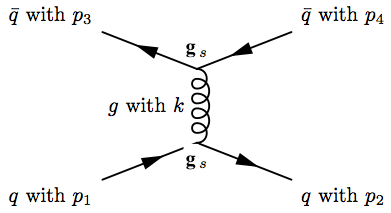
\includegraphics[width=0.5\textwidth]{fig/strongforce/strong_mom_transf.png}
\end{center}
The energy scale of the interaction is determined by the momentum transfer $k$ from the initial to the final state and is given by
\[
k=(p_2-p_1)=(p_4-p_3)
\]
At low momentum transfer (or energy scale) the strong force has a coupling strength close to 1. However at higher energies the strength of the strong force decreases. This means that at low energies, quarks form bound states as they interact strongly via gluon field. We call this effect ``Asymptotic freedom''. In fact at an energy transfer $k^2\sim M_{Z^0}^2\sim 90^2$~GeV$^2$, $\alpha_s\sim0.12$!.
\begin{center}
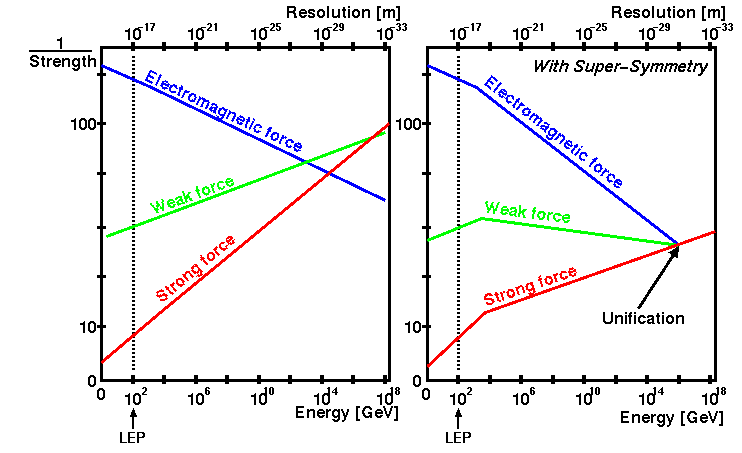
\includegraphics[width=0.8\textwidth]{fig/strongforce/running_coupling.png}
\end{center}
As an aside, it is interesting to consider the fact that all the coupling constants at some energy scale could all have the same value. This is the concept behind unifying all forces. At some energy scale all forces in nature become part of a single interaction. However the Standard Model of particle physics does not predict a unification of all forces (it does however offer a way of unifying the Weak and Electromagnetic forces). However extensions to the Standard Model, such as Supersymmetry, can offer a way of unifying these three forces at a high energy scale.
